\documentclass[../main.tex]{subfiles}

\begin{document}

\chapter{ОГЛЯД ТА АНАЛІЗ ЗАСОБІВ ПРОЕКТУВАННЯ ТА РОЗРОБКИ ANDROID-ЩОДЕННИКА}

\section{Призначення та область застосування об'єкта проектування}

Люди, які часто подорожують, відвідують багато різних місць, зустрічаються з новими людьми, переживають нові ситуації. Деякі події залишаються в пам'яті, деякі відходять на другий план попри небажання їх~забути. Інформація накопичується, а людина не~в~змозі запам'ятати все. Тому, необхідність збереження пам'яті про деякі події, місця чи враження зумовлює створення систем для задоволення таких потреб.

Об'єктом проектування є щоденник, а призначення щоденників полягає в тому, щоб зберігати записи за певний період часу. Оскільки щоденник призначений для мобільних пристроїв, його можна з легкістю використовувати в дорозі. Попри те, що цільовою аудиторією є~мандрівники, використовувати розроблюваний додаток можуть і ті, хто просто бажає вести свій щоденник. Також можна використовувати його тільки для запису треку чи нагадувань.

\section{Способи та засоби реалізації}

Android -- це операційна система для мобільних пристроїв та~планшетних комп'ютерів, створена компанією Google. Базується на ядрі Linux, проте стоїть дещо осторонь від спільноти та інфраструктури Linux. Базовим елементом цієї операційної системи є реалізація Dalvik віртуальної машини Java, все програмне забезпечення та застосування спираються на~цю реалізацію Java.

Додатки для Android зазвичай пишуться мовою програмування Java. Інструменти Android SDK (Software Development Kit -- комплект розробки програмного забезпечення) компілюють написаний код і всі необхідні файли даних та ресурсів у файл APK (програмний пакет Android), який являє собою файл архіву з розширенням .apk. У файлі APK знаходиться все, що потрібно для роботи Android-додатку, і він дозволяє встановити додаток на будь-якому пристрої під управлінням системи Android \cite{android_for_devs}. 

Також існує Android NDK (Native Development Kit), що являє собою набір інструментів, який дозволяє використовувати код на C і C++ з~Android, а також надає бібліотеки платформи, які можна використовувати для управління нативними діяльностями та для доступу до фізичних компонентів пристрою, таких як датчики та сенсорний ввід. NDK може не~підходити для більшості початківців, якщо їм потрібно використовувати тільки Java код та API-інтерфейси для розробки своїх додатків. Проте, NDK може бути корисним в тих випадках, коли потрібно зробити одну або декілька з наступних дій:

\begin{enumerate}
	\item Отримати додаткову продуктивність для пристрою, щоб зменшити час затримки, або для запуску обчислювально-інтенсивних додатків, таких як ігри або фізичне моделювання.
	\item Повторно використовувати бібліотеки (власні або інших розробників), що написані на C чи C++.
\end{enumerate}

Оскільки розроблюваний додаток не являється грою та немає потреби у~використанні бібліотек на C/C++, для його розробки можна використовувати такі мови, як Java, Kotlin, Scala чи Groovy.

\subparagraph{Scala.}
Мультипарадигмова мова програмування Scala спроектована короткою та типобезбечною для простого і швидеого створення компонентного програмного забезпечення, поєднує в собі властивості об'єктно-орієнтованого та функціонального програмування. 

Перші версії мови створені в 2003 році колективом лабораторії методів програмування Федеральної політехнічної школи Лозанни під керівництвом Мартіна Одерски, мова реалізована для платформ Java та .Net. На думку Джеймса Стречена, творця мови програмування Groovy, Scala може стати наступником мови Java.

Scala-програми багато в чому схожі на Java-програми, і можуть вільно взаємодіяти з Java-кодом. Мова включає однакову об'єктну модель -- в тому сенсі, що будь-яке значення є об'єктом, а будь-яка операція -- викликом методу. При цьому є функціональною мовою, функції -- це повноправні значення.

В Scala включені потужні і одноманітні концепції абстракцій як для типів, так і для значень. Зокрема, вона містить гнучкі симетричні конструкції домішок для композиції класів і типажів. Дозволяє здійснювати декомпозицію об'єктів шляхом порівняння зі зразком; зразки і вирази при цьому були узагальнені для підтримки природної обробки \mbox{XML-документів}. В цілому, ці конструкції дозволяють легко виражати самостійні компоненти, які використовують бібліотеки Scala, не~користуючись спеціальними мовними конструкціями~\cite{scala}.

Мова допускає зовнішні розширення компонентів за допомогою представлень (views). Можливості узагальненого програмування реалізуються внаслідок підтримки узагальнених функцій (generics), у тому числі вищого типажу (generics of a higher kind). Крім різних класичних структурних типів даних, в мову включена підтримка екзистенціальних типів.

\subparagraph{Groovy.}
Об'єктно-орієнтована мова програмування Groovy розроблена для платформи Java як доповнення до мови Java з~можливостями Python, Ruby і Smalltalk. Groovy використовує Java-подібний синтаксис з динамічною компіляцією в JVM байт-код і~безпосередньо працює з іншим Java кодом і бібліотеками. Мова може використовуватися в~будь-якому Java-проекті або як скриптова мова. 

Можливості Groovy що відрізняють її від Java:
\begin{itemize}[label={--}]
	\item статична та динамічна типізація;
	\item вбудований синтаксис для списків, асоціативних масивів, масивів і~регулярних виразів;
	\item замикання;
	\item перевантаження операцій.
\end{itemize}

В програмуванні, замиканням (closure) називається підпрограма, що~виконується в середовищі, що містить одну або більше зв'язаних змінних. Під час виконання, підпрограма має доступ до цих змінних. Застосування замикань асоціюється з функціональним програмуванням. Такі конструкції, як об'єкти в інших мовах програмування, у~функціональному програмуванні можуть моделюватись із допомогою замикань~\cite{groovy}.

Останнім часом Groovy разом з Grails (програмний каркас для створення веб-застосунків) стали популярними технологіями. Приймаючи рішення про те, чи варто використовувати їх у якомусь конкретному випадку потрібно пам’ятати про динамічну спрямованість мови та~використовувати там, де потрібно використовувати саме динамічні мови. Там де потрібна надійність або значна швидкодія рекомендується використовувати статичні мови, зокрема Java чи Scala. Адже відомо, що~зробити помилку при розробці в першому випадку значно легше.

\subparagraph{Kotlin.}
Мова програмування Kotlin -- це статично типізована мова програмування, що працює поверх JVM і розробляється компанією JetBrains. Компілюється також в JavaScript і на інші платформи. Мова названа на честь острова Котлін у Фінській затоці, на якому розташоване місто Кронштадт. Автори ставили за мету створити мову більш лаконічну і типобезпечнішу, ніж Java, і більш просту, ніж Scala~\cite{open_systems}. Наслідками спрощення в порівнянні зі~Scala стали також швидша компіляція та краща підтримка мови в~середовищі розробки.

Позиціонується розробниками як об'єктно-орієнтована мова промислового рівня, а також як мова, яка зможе замінити Java. При цьому вона повністю сумісна з Java, що дозволяє розробникам поступово перейти з Java на Kotlin. Зокрема, в Android мова інтегрується за допомогою Gradle, що дозволяє впроваджувати нові функції на Kotlin для існуючого Android-додатку без повного переписування програми.

\subparagraph{Java.}
Мова програмування Java являє собою об'єктно-орієнтовану мову, що розробляється компанією Sun Microsystems з 1991 року та офіційно випущена 23 травня 1995 року. Спочатку ця мова програмування  мала назву Oak (James Gosling) і розроблялася для побутової електроніки, але згодом була перейменована в Java і стала використовуватися для написання аплетів, додатків і серверного програмного забезпечення.

Програми, написані на Java, можуть бути трансльовані в байт-код, що~виконується на віртуальній java-машині (JVM) -- програмі, що обробляє байт-код і передає інструкції обладнанню, як інтерпретатор, але байт-код, на відміну від тексту, обробляється значно швидше~\cite{learn_java}.

Три ключові елементи об'єднались в технології мови Java:
\begin{enumerate}
	\item Широке використання аплетів (applets) -- невеликих активних мережевих додатків, що не залежать від платформи та вбудовуються в~web-сторінки. Аплети Java можуть налаштовуватися та~поширюватися споживачам з такою ж легкістю, як будь-які документи HTML.
	\item Java надає можливість об'єктно-орієнтованої розробки додатків, поєднуючи простий і знайомий синтаксис з надійним і зручним в~роботі середовищем розробки. Це дозволяє широкому колу програмістів швидко створювати нові програми та аплети.
	\item Надає програмісту багатий набір класів для ясного абстрагування багатьох системних функцій, що використовуються при роботі з~вікнами чи мережею. Ключовою характеристикою цих класів є те, що~вони забезпечують створення незалежних від використовуваної платформи абстракцій для широкого спектра системних інтерфейсів.
\end{enumerate}

Весь набір функцій в операційній системі Android доступний через API-інтерфейси, що написані на мові Java. Ці API утворюють будівельні блоки, необхідні для створення додатків для Android, спрощуючи повторне використання ядра, модульних компонентів та системних служб, які містять наступне:

\begin{enumerate}
	\item Багату і розширювану систему виглядів (View System), яку можна використовувати для створення інтерфейсу користувача додатку, в~тому числі списки, сітки, текстові поля, кнопки і, навіть, вбудовуваний веб-браузер.
	\item Менеджер ресурсів, що забезпечує доступ до ресурсів, таких як~локалізовані рядкові ресурси, графіка та файли макетів (layout files).
	\item Менеджер повідомлень, який дозволяє всім додаткам показувати призначені для користувача повідомлення в рядку стану.
	\item Менеджер активності, який керує життєвим циклом додатків і надає загальну систему навігації (navigation back stack).
	\item Контент-провайдери, які дозволяють додаткам отримувати доступ до~даних з інших додатків, або ділитися своїми власними даними.
\end{enumerate}

Розробники мають повний доступ тих самих API-інтерфейсів, що~використовуються в системних Android додатках.

Оскільки Android API базується на принципах об'єктно-орієнтованого програмування, написання Android додатку неможливе без використання цього підходу. Об'єктно-орієнтоване програмування (ООП) -- методологія програмування, заснована на представленні програми у вигляді сукупності об'єктів, кожен з яких є екземпляром певного класу, а класи утворюють ієрархію спадкування~\cite{oop}.

Основними механізмами об'єктно-орієнтованого програмування є:
\begin{enumerate}
	\item Інкапсуляція -- це властивість системи, що дозволяє об'єднати дані та~методи, що працюють з ними, в класі й приховати деталі реалізації від користувача.
	\item Наслідування -- властивість, що дозволяє описати новий клас на~основі вже існуючого, частково або повністю запозичуючи його функціональність. Клас, від якого відбувається наслідування, називається базовим або батьківським. Новий клас -- нащадком, спадкоємцем або похідним класом.
	\item Поліморфізм -- здатність використовувати об'єкти з однаковим інтерфейсом без інформації про тип і внутрішню структуру об'єкта.
\end{enumerate}

Також, іноді виділяють абстрагування -- спосіб виділити набір значущих характеристик об'єкта, виключаючи з розгляду незначущі. Відповідно, абстракція -- це набір всіх таких характеристик.

\subparagraph{Android Studio.}
Найпопулярнішим та офіційним середовищем розробки для Android є Android Studio. Вона являє собою інтегроване середовище розробки (IDE) для роботи з платформою Android, анонсована 16 травня 2013 року на конференції Google I/O. Перебувала у вільному доступі починаючи з версії 0.1, що була опублікована в травні 2013 року, а~потім перейшла в стадію бета-тестування, починаючи з версії 0.8, яка була випущена в червні 2014 року. Перша стабільна версія 1.0 була випущена в~грудні 2014 року, тоді ж припинилася підтримка модуля Android Development Tools (ADT) для середовища розробки Eclipse.

Android Studio ґрунтується на програмному забезпеченні IntelliJ IDEA від компанії JetBrains. Дане середовище розробки доступне для Windows, OS~X і Linux~\cite{android_studio}. Воно дозволяє швидко та зручно писати код, збирати проекти за допомогою Gradle (система автоматичного збирання, побудована на принципах Apache Ant і Apache Mave).

Останнім часом для збереження даних в Android-додатках активно використовують бази даних noSQL, такі як Realm чи Firebase. NoSQL прибирає всі обмеження реляційної моделі (недостатня продуктивність, трудомістке горизонтальне масштабування) і полегшує засоби зберігання та доступу до даних. Такі БД використовують неструктурований підхід (створення структури на льоту), тим самим знімаючи обмеження жорстких зв'язків і пропонуючи різні типи доступу до специфічних даних~\cite{nosql}. В~нашому випадку актуальним вибором є Firebase, оскільки вона являє собою базу даних, яка в реальному часі поновлює інформацію на всіх з'єднаних з~нею пристроях, що забезпечує синхронізацію між пристроями. Також плюсом цієї БД є те, що вона зберігає дані оффлайн на пристрої, тому при втраті інтернет з'єднання всі дані будуть збережені й вивантажені при його відновленні.

Для авторизації користувачів в додатку зручним та актуальним способом є авторизація за допомогою Google-акаунта. Більшість Android користувачів мають його, тому їм не доведеться створювати нові акаунти та~запам'ятовувати новий пароль.

Однією з унікальних особливостей мобільних додатків є обізнаність про місцезнаходження. Користувачі мобільних пристроїв беруть свої пристрої з собою повсюди, і додавання інформації про місцезнаходження в~додаток приносить користувачам більш контекстний досвід. 

Всі сучасні смартфони обладнані GPS-приймачем, тому вони можуть виступати в ролі трекера.  Як окремий пристрій GPS-трекер являє собою прилад прийому-передачі даних для супутникового контролю автомобілів, людей чи інших об'єктів, до яких він прикріплюється, що використовує GPS для точного визначення місцезнаходження об'єкта. Глобальна система позиціонування (GPS) – супутникова система навігації, що забезпечує вимір відстані, часу та визначає місцезнаходження у всесвітній системі координат WGS~84~\cite{gps}. Дозволяє в будь-якому місці Землі визначати місцезнаходження та швидкість об'єктів. Вона також потрібна для реалізації нагадувань по приближенню до заданого місця.

Для Android доступні API для роботи з місцезнаходженням, вони знаходяться в сервісах Google Play та полегшують роботу з інформацією про місцезнаходження, автоматизованим відстеженням розташування та~визнанням активності. 

Також, існує \textit{Google Maps Android API}. Вона дозволяє додавати карти та налаштовувати їх відображення в додатку: відмічання локацій за~допомогою власних маркерів, розширення картографічних даних за~допомогою накладання зображень, вбудовування однієї або декількох карт як фрагментів та багато іншого~\cite{google_maps}.

\section{Аналіз переваг та недоліків програм аналогів}

{
%\clubpenalty=10000 % to avoid (surely) situation when only first line of paragraph remains on current page but all others go to next page

\widowpenalties=3 10000 10000 150 % line above doesn't work

Ключовим моментом початку розробки є пошук, аналіз та порівняння аналогічних або подібних по тематиці програмних продуктів. Потрібно визначити, які плюси та мінуси є у вже існуючих додатків з точки зору користувача.

Існує багато різноманітних додатків, які являють собою Android-щоденники для мандрівників, розглянемо більш детально основні з них. Для пошуку додатків правильним рішенням буде використовувати Google Play -- офіційний магазин додатків від Google. Він містить як платні, так і безкоштовні додатки, які розміщені за певними категоріями. В~нашому випадку категорією для пошуку додатків буде категорія подорожей.

Першим розглянутим продуктом є Journey - Diary, Journal від розробника Two App Studio Pte. Ltd. Додаток містить обов'язкову авторизацію за допомогою облікового запису Google. Можна створювати записи, вказувати для них теги та додавати до 4-х фото. При вказанні локації автоматично завантажуються дані про погоду. Також можна вказувати активність (непорушний, біг, політ і т. д.). Для користування можливостями розмітки «Markdown» потрібно купувати преміум-акаунт. Головний екран додатку містить список записів (рис. \ref{figure:1.1}). Присутній пошук, але він фільтрує тільки по тексту запису. Синхронізація даних відбувається через Google Drive (сховище даних, що дозволяє користувачам зберігати свої дані на серверах у хмарі і ділитися ними з іншими користувачами в Інтернеті). Також є можливість поділитися та~опублікувати запис. 

\begin{figure}[H]
\centering
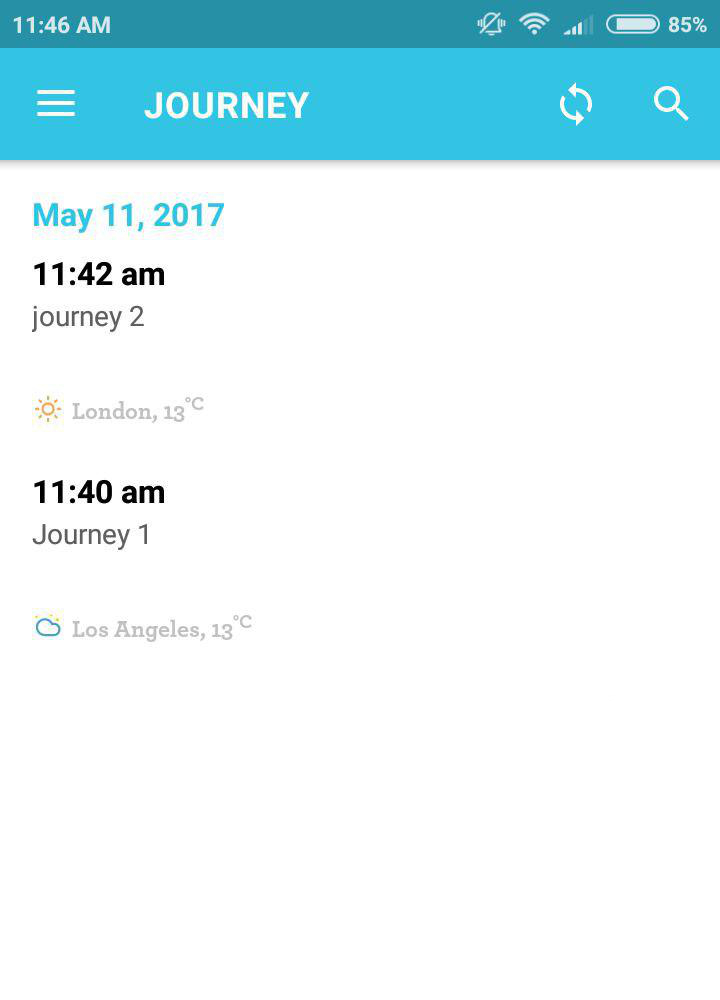
\includegraphics[width=0.5\textwidth]{journey_main_screen}
\caption{Головний екран додатку Journey - Diary, Journal}
\label{figure:1.1}
\end{figure}

Другим додатком є The Traveler від розробника 14Eleven Development LLC. Авторизація відбувається за допомогою облікового запису Google. Можна також синхронізувати дані про активність з додатком Google Fit. Можна створювати подорожі та записувати трек. Щоденник, як такий, відсутній, можна додавати медіа файли та пов'язувати їх зі шляхами. Шляхи можна переглядати на карті та експортувати. Завантажувати подорожі до хмарного сервісу чи ділитися ними можна лише в платній версії додатку. Головний екран містить дві вкладки зі списками поточних та~минулих подорожей (рис. \ref{figure:1.2}). 

\begin{figure}[H]
	\centering
	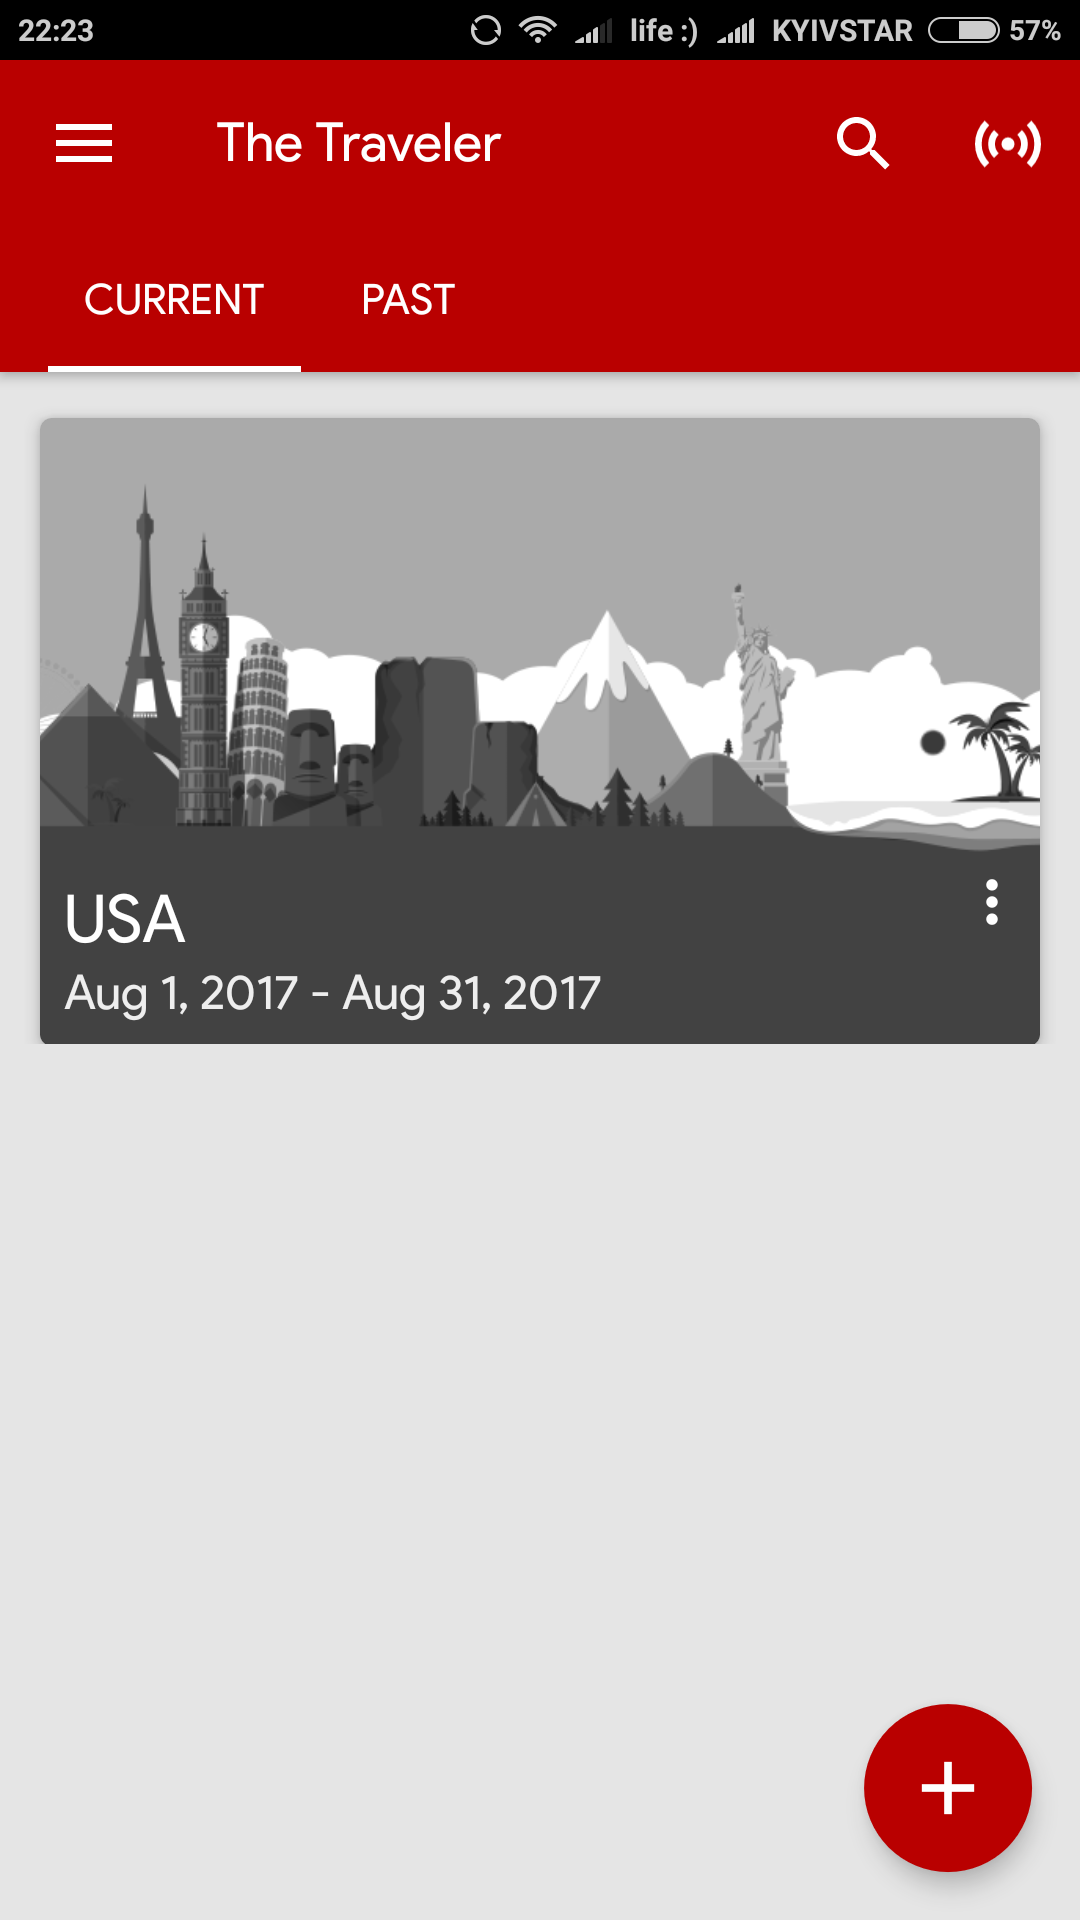
\includegraphics[width=0.5\textwidth]{the_traveler_main_screen}
	\caption{Головний екран додатку The Traveler}
	\label{figure:1.2}
\end{figure}

Наступним продуктом є Travel Diary від розробника Tristan Rücker. Додаток являє собою записник, в якому можна створювати категорії (подорожі). Головний екран містить список цих подорожей (рис. \ref{figure:1.3}). Логотип подорожі користувач вказує сам, обираючи один із трьох доступних. В категоріях можна робити записи, прикріпляти до них фото та~вказувати локації. Ці записи можна експортувати в pdf-файли, надсилати через електронну пошту. Також можна переглядати вказані локації на карті, але лише для одного запису. Присутнє сортування записів за датою та~назвою.

\begin{figure}[H]
\centering
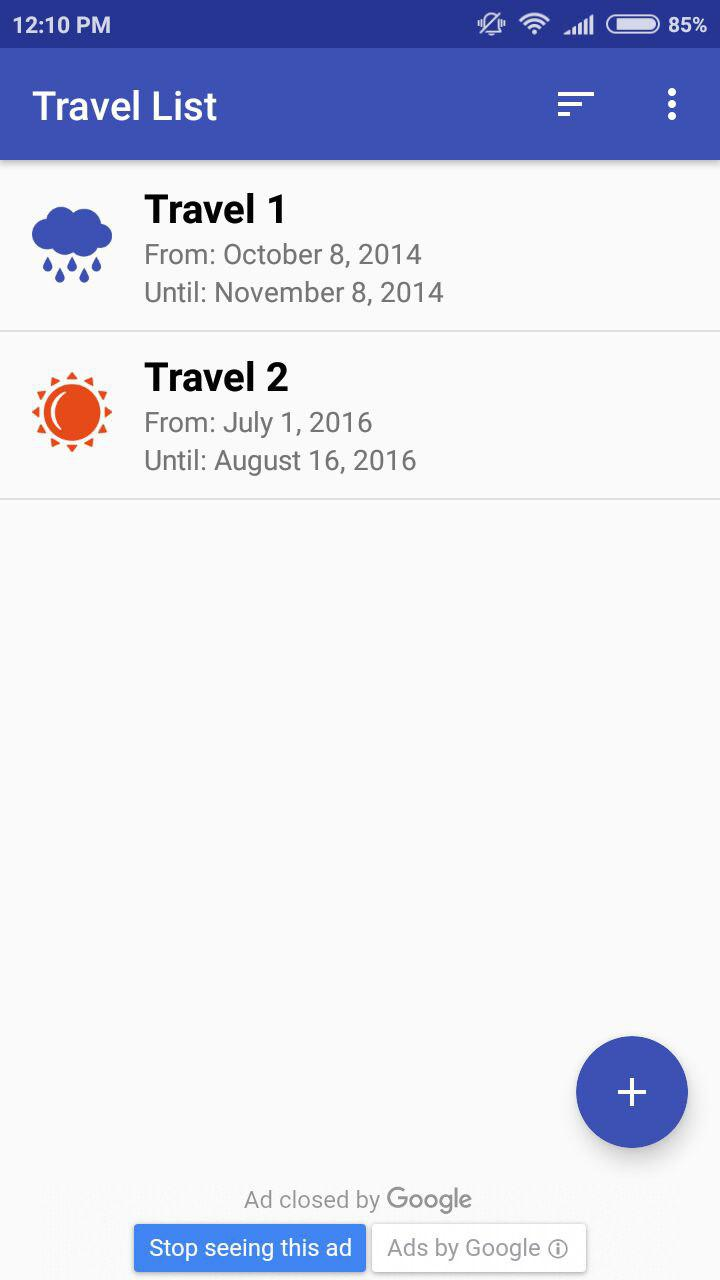
\includegraphics[width=0.5\textwidth]{travel_diary_main_screen}
\caption{Головний екран додатку Travel Diary}
\label{figure:1.3}
\end{figure}

Ще одним розглянутим продуктом є Universal diary від розробника SPB Apps. Головний екран містить календар, потрібно обрати дату для того щоб продовжити (рис. \ref{figure:1.4}). Після обрання дати можна створювати записи, так звані мітки дня. Міткою дня може бути текст, фото, задача чи фінанси. Можливе створення резервної копії на Google Drive чи на карті пам'яті. При спробі виходу з додатка декілька разів показується реклама.

\begin{figure}[H]
\centering
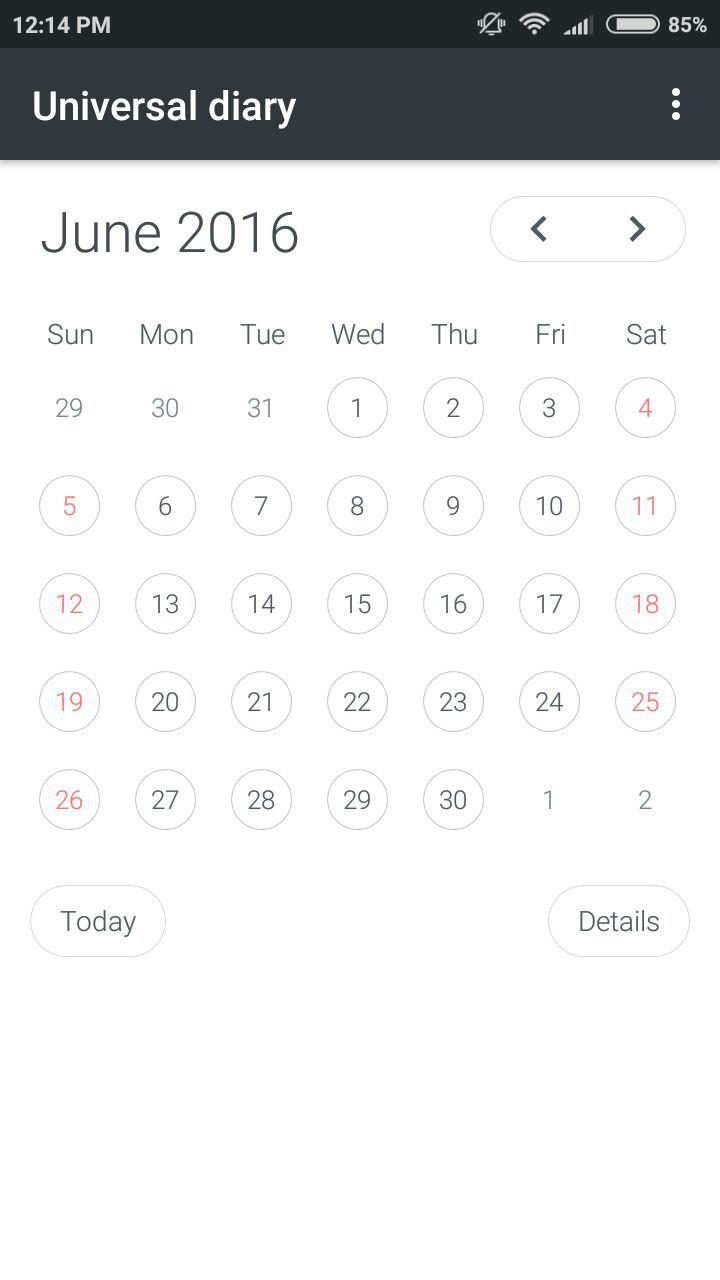
\includegraphics[width=0.5\textwidth]{universal_diary_main_screen}
\caption{Головний екран додатку Universal diary}
\label{figure:1.4}
\end{figure}

Отже, порівняння основних функцій додатків аналогів та додатку за~темою дипломної роботи буде виглядати так, як вказано в таблиці \ref{table:1.1}.

\begin{tableJustNowSureWholeOnSamePage}
\footnotesize
\captionof{table}{Порівняльна таблиця основних функцій існуючих додатків аналогів}
\begin{tabular}{ |p{2.5cm}|p{2cm}|p{2.5cm}|p{2.5cm}|p{2.5cm}|p{2.5cm}| } 
    \hline
    \thead{Назва} &
    \thead{Щоденник} &
    \thead{Нагадування\\за часом} &
    \thead{Нагадування\\за місцем} &
    \thead{Запис треку\\переміщень} &
    \thead{Синхронізація} \\
    \hline
    Journey &
    \thead{+} &
    & & &
    \thead{+} \\
    \hline
    The Traveler &
    & & & 
    \thead{+} & \\
    \hline
    Travel Diary &
    \thead{+} &
    & & & \\    
    \hline
    Universal diary &
    \thead{+} &
    \thead{+} & 
    & & \\
    \hline
    Розроблюваний додаток &
    \thead{+} &
    \thead{+} & 
    \thead{+} & 
    \thead{+} & 
    \thead{+} \\
    \hline
\end{tabular}
\label{table:1.1}
\end{tableJustNowSureWholeOnSamePage}

Порівняємо також додаткові функції цих додатків. Результати представлено в таблиці \ref{table:1.2}.

\begin{tableJustNowSureWholeOnSamePage}
\footnotesize
\captionof{table}{Порівняльна таблиця додаткових функцій існуючих додатків аналогів}
\begin{tabular}{ |p{2.5cm}|p{2.5cm}|p{2.5cm}|p{2.5cm}|p{2cm}|p{2.5cm}| } 
    \hline
    \thead{Назва} &
    \thead{Додавання\\фото} &
    \thead{Місце\\свотрення\\запису} &
    \thead{Збереження\\погодних умов} &
    \thead{Експорт\\записів} &
    \thead{Створення\\резервної копії} \\
    \hline
    Journey &
    \thead{+} &
    \thead{+} & 
    \thead{+} & 
    \thead{+} & \\
    \hline
    The Traveler &
    \thead{+} &
    \thead{+} & 
    & & \\
    \hline
    Travel Diary &
    \thead{+} &
    \thead{+} &
    & & 
    \thead{+} \\    
    \hline
    Universal diary &
    \thead{+} &
    & & & 
    \thead{+}\\
    \hline
    Розроблюваний додаток &
    \thead{+} &
    \thead{+} & 
    \thead{+} & 
    & \\
    \hline
\end{tabular}
\label{table:1.2}
\end{tableJustNowSureWholeOnSamePage}

Порівнявши функції додатків, бачимо, що розроблюваний додаток об'єднує в собі як функції які є окремо в додатках аналогах, так і додаткові, такі як запис треку, чи нагадування за місцем. Також значним плюсом є~відсутність реклами.

}

\section{Задача розробки}

Програмних продуктів, які дозволяють вести щоденник, досить велика кількість. Існують також додатки окремо для запису треку переміщень чи встановлення нагадувань, але продуктів, що поєднують в~собі ці функції не так багато. Для поєднання цих функцій, майбутній продукт повинен задовольняти такі вимоги: 

\begin{enumerate}
	\item Можливість створення/редагування/видалення подорожі.
	\item Можливість створення/редагування/видалення запису щоденника та~планувальника.
	\item Можливість додавання/видалення фото в записі щоденника.
	\item Зберігання погодних умов та місця створення запису.
	\item Можливість ділитися записом щоденника та окремими фото.
	\item Можливість запису треку переміщень та перегляду його на карті.
	\item Можливість створення/редагування/видалення списку завдань та~нагадувань (планувальника).
\end{enumerate}

Практичною цінністю майбутнього додатку є надання комплексу інструментів для допомоги в організації та збереженні вражень від подорожей чи плануванні майбутніх поїздок.

\section{Висновки}

{
\widowpenalties=3 10000 10000 150  % у методичці (розд.6.3) сказано "Не допускається розміщувати назву розділу, підрозділу, а також пункту й підпункту в нижній частині сторінки, якщо після цього текст займає до двох рядків." На жаль, не~вмію зробити так, щоб ці заборони були ТІЛЬКИ після заголовків, а робити таке у преамбулі абсолютно для вісх абзаців теж ніби погано.

Визначено призначення та область застосування Android-щоденника, проведено огляд способів та засобів його реалізації. Проведено аналіз існуючих програмних аналогів, та зроблено висновок про практичну цінність та актуальність його розробки.

}

Результатом виконання цього розділу є формування задачі розробки Android-щоденника для мандрівників, визначення вимог, які він повинен задовольняти з урахуванням переваг та недоліків існуючих програмних продуктів у даній галузі. Було визначено, що додаток повинен мати авторизацію користувачів за допомогою облікового запису Google. Також, користувач повинен мати можливість працювати з подорожами, записами щоденника чи планувальника, встановлювати нагадування та записувати трек переміщень.

\end{document}
